% 자동 생성물 — 손으로 고치지 말 것.
% 출처: accounting-scatter.svg (docs/paper2/figures/make_figures.py 생성)
% 생성: python docs/paper2/figures/svg_to_tikz.py --width-pt 240
% 본문 삽입용. 논문 문서에서 \input 하면 글자가 본문 폰트로 조판된다.
\definecolor{accountingscc0}{HTML}{FFFFFF}
\definecolor{accountingscc1}{HTML}{69737D}
\definecolor{accountingscc2}{HTML}{17212B}
\definecolor{accountingscc3}{HTML}{DCE2E8}
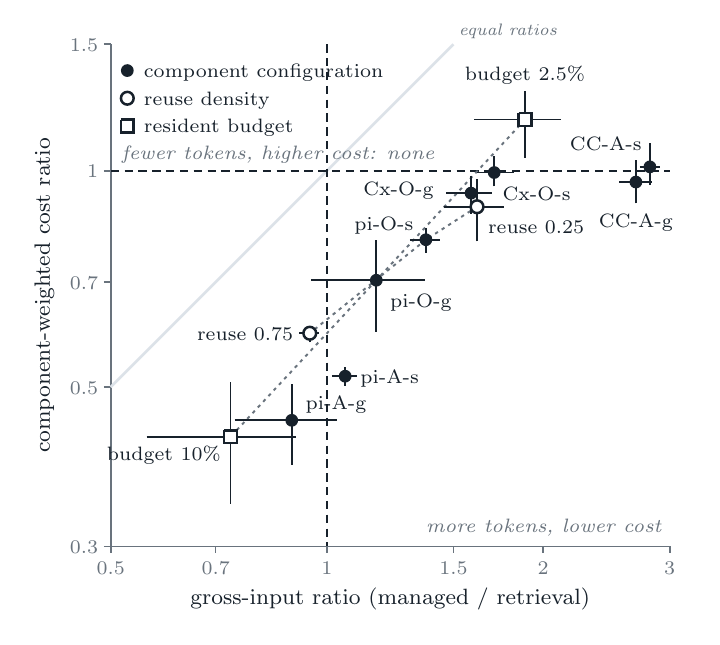
\begin{tikzpicture}[baseline]
\useasboundingbox (0.000pt,0.000pt) rectangle (240.000pt,213.000pt);
\fill[accountingscc0] (0.000pt,0.000pt) rectangle (240.000pt,213.000pt);
\draw[accountingscc1, line width=0.600pt] (30.000pt,25.550pt) -- (232.000pt,25.550pt);
\draw[accountingscc1, line width=0.600pt] (30.000pt,207.000pt) -- (30.000pt,25.550pt);
\draw[accountingscc1, line width=0.600pt] (30.000pt,25.550pt) -- (30.000pt,23.050pt);
\node[anchor=base, accountingscc1, font=\fontsize{7.50pt}{9.00pt}\selectfont, inner sep=0pt, outer sep=0pt] at (30.000pt,15.550pt) {0.5};
\draw[accountingscc1, line width=0.600pt] (67.930pt,25.550pt) -- (67.930pt,23.050pt);
\node[anchor=base, accountingscc1, font=\fontsize{7.50pt}{9.00pt}\selectfont, inner sep=0pt, outer sep=0pt] at (67.930pt,15.550pt) {0.7};
\draw[accountingscc1, line width=0.600pt] (108.140pt,25.550pt) -- (108.140pt,23.050pt);
\node[anchor=base, accountingscc1, font=\fontsize{7.50pt}{9.00pt}\selectfont, inner sep=0pt, outer sep=0pt] at (108.140pt,15.550pt) {1};
\draw[accountingscc1, line width=0.600pt] (153.860pt,25.550pt) -- (153.860pt,23.050pt);
\node[anchor=base, accountingscc1, font=\fontsize{7.50pt}{9.00pt}\selectfont, inner sep=0pt, outer sep=0pt] at (153.860pt,15.550pt) {1.5};
\draw[accountingscc1, line width=0.600pt] (186.290pt,25.550pt) -- (186.290pt,23.050pt);
\node[anchor=base, accountingscc1, font=\fontsize{7.50pt}{9.00pt}\selectfont, inner sep=0pt, outer sep=0pt] at (186.290pt,15.550pt) {2};
\draw[accountingscc1, line width=0.600pt] (232.000pt,25.550pt) -- (232.000pt,23.050pt);
\node[anchor=base, accountingscc1, font=\fontsize{7.50pt}{9.00pt}\selectfont, inner sep=0pt, outer sep=0pt] at (232.000pt,15.550pt) {3};
\draw[accountingscc1, line width=0.600pt] (27.500pt,25.550pt) -- (30.000pt,25.550pt);
\node[anchor=base east, accountingscc1, font=\fontsize{7.50pt}{9.00pt}\selectfont, inner sep=0pt, outer sep=0pt] at (25.500pt,22.950pt) {0.3};
\draw[accountingscc1, line width=0.600pt] (27.500pt,83.140pt) -- (30.000pt,83.140pt);
\node[anchor=base east, accountingscc1, font=\fontsize{7.50pt}{9.00pt}\selectfont, inner sep=0pt, outer sep=0pt] at (25.500pt,80.540pt) {0.5};
\draw[accountingscc1, line width=0.600pt] (27.500pt,121.080pt) -- (30.000pt,121.080pt);
\node[anchor=base east, accountingscc1, font=\fontsize{7.50pt}{9.00pt}\selectfont, inner sep=0pt, outer sep=0pt] at (25.500pt,118.480pt) {0.7};
\draw[accountingscc1, line width=0.600pt] (27.500pt,161.290pt) -- (30.000pt,161.290pt);
\node[anchor=base east, accountingscc1, font=\fontsize{7.50pt}{9.00pt}\selectfont, inner sep=0pt, outer sep=0pt] at (25.500pt,158.690pt) {1};
\draw[accountingscc1, line width=0.600pt] (27.500pt,207.000pt) -- (30.000pt,207.000pt);
\node[anchor=base east, accountingscc1, font=\fontsize{7.50pt}{9.00pt}\selectfont, inner sep=0pt, outer sep=0pt] at (25.500pt,204.400pt) {1.5};
\node[anchor=base, accountingscc2, font=\fontsize{8.00pt}{9.60pt}\selectfont, inner sep=0pt, outer sep=0pt] at (131.000pt,4.550pt) {gross-input ratio (managed / retrieval)};
\node[anchor=base, accountingscc2, font=\fontsize{8.00pt}{9.60pt}\selectfont, inner sep=0pt, outer sep=0pt, rotate=90] at (8.000pt,116.280pt) {component-weighted cost ratio};
\draw[accountingscc3, line width=0.900pt] (30.000pt,83.140pt) -- (153.860pt,207.000pt);
\node[anchor=base west, accountingscc1, font=\fontsize{6.50pt}{7.80pt}\selectfont, inner sep=0pt, outer sep=0pt] at (155.860pt,210.000pt) {\itshape equal ratios};
\draw[accountingscc2, line width=0.800pt, dash pattern=on 3.00pt off 2.00pt] (108.140pt,207.000pt) -- (108.140pt,25.550pt);
\draw[accountingscc2, line width=0.800pt, dash pattern=on 3.00pt off 2.00pt] (30.000pt,161.290pt) -- (232.000pt,161.290pt);
\node[anchor=base west, accountingscc1, font=\fontsize{7.00pt}{8.40pt}\selectfont, inner sep=0pt, outer sep=0pt] at (34.000pt,165.290pt) {\itshape fewer tokens, higher cost: none};
\node[anchor=base east, accountingscc1, font=\fontsize{7.00pt}{8.40pt}\selectfont, inner sep=0pt, outer sep=0pt] at (229.000pt,30.550pt) {\itshape more tokens, lower cost};
\draw[accountingscc1, line width=0.700pt, dash pattern=on 1.20pt off 1.60pt] (162.370pt,148.290pt) -- (143.900pt,136.370pt);
\draw[accountingscc1, line width=0.700pt, dash pattern=on 1.20pt off 1.60pt] (143.900pt,136.370pt) -- (101.940pt,102.590pt);
\draw[accountingscc1, line width=0.700pt, dash pattern=on 1.20pt off 1.60pt] (179.710pt,179.780pt) -- (125.970pt,121.730pt);
\draw[accountingscc1, line width=0.700pt, dash pattern=on 1.20pt off 1.60pt] (125.970pt,121.730pt) -- (73.290pt,65.140pt);
\draw[accountingscc2, line width=0.600pt] (213.770pt,157.210pt) -- (225.470pt,157.210pt);
\draw[accountingscc2, line width=0.600pt] (219.780pt,149.490pt) -- (219.780pt,165.140pt);
\draw[accountingscc2, line width=0.600pt] (221.210pt,162.700pt) -- (228.310pt,162.700pt);
\draw[accountingscc2, line width=0.600pt] (224.840pt,156.230pt) -- (224.840pt,171.220pt);
\draw[accountingscc2, line width=0.600pt] (74.790pt,71.120pt) -- (111.740pt,71.120pt);
\draw[accountingscc2, line width=0.600pt] (95.430pt,55.140pt) -- (95.430pt,84.330pt);
\draw[accountingscc2, line width=0.600pt] (102.550pt,121.730pt) -- (143.420pt,121.730pt);
\draw[accountingscc2, line width=0.600pt] (125.970pt,103.070pt) -- (125.970pt,136.100pt);
\draw[accountingscc2, line width=0.600pt] (109.920pt,87.060pt) -- (119.100pt,87.060pt);
\draw[accountingscc2, line width=0.600pt] (114.720pt,83.600pt) -- (114.720pt,90.230pt);
\draw[accountingscc2, line width=0.600pt] (138.140pt,136.370pt) -- (148.950pt,136.370pt);
\draw[accountingscc2, line width=0.600pt] (143.900pt,131.710pt) -- (143.900pt,140.540pt);
\draw[accountingscc2, line width=0.600pt] (151.310pt,153.210pt) -- (167.620pt,153.210pt);
\draw[accountingscc2, line width=0.600pt] (160.210pt,145.780pt) -- (160.210pt,159.460pt);
\draw[accountingscc2, line width=0.600pt] (162.300pt,160.650pt) -- (175.870pt,160.650pt);
\draw[accountingscc2, line width=0.600pt] (168.580pt,155.660pt) -- (168.580pt,166.800pt);
\draw[accountingscc2, line width=0.600pt] (150.310pt,148.290pt) -- (172.290pt,148.290pt);
\draw[accountingscc2, line width=0.600pt] (162.370pt,135.770pt) -- (162.370pt,158.340pt);
\draw[accountingscc2, line width=0.600pt] (98.190pt,102.590pt) -- (105.220pt,102.590pt);
\draw[accountingscc2, line width=0.600pt] (101.940pt,99.320pt) -- (101.940pt,105.290pt);
\draw[accountingscc2, line width=0.600pt] (161.290pt,179.780pt) -- (192.780pt,179.780pt);
\draw[accountingscc2, line width=0.600pt] (179.710pt,166.000pt) -- (179.710pt,190.180pt);
\draw[accountingscc2, line width=0.600pt] (43.020pt,65.140pt) -- (96.980pt,65.140pt);
\draw[accountingscc2, line width=0.600pt] (73.290pt,41.040pt) -- (73.290pt,84.880pt);
\fill[accountingscc2] (219.780pt,157.210pt) circle[radius=2.300pt];
\fill[accountingscc2] (224.840pt,162.700pt) circle[radius=2.300pt];
\fill[accountingscc2] (95.430pt,71.120pt) circle[radius=2.300pt];
\fill[accountingscc2] (125.970pt,121.730pt) circle[radius=2.300pt];
\fill[accountingscc2] (114.720pt,87.060pt) circle[radius=2.300pt];
\fill[accountingscc2] (143.900pt,136.370pt) circle[radius=2.300pt];
\fill[accountingscc2] (160.210pt,153.210pt) circle[radius=2.300pt];
\fill[accountingscc2] (168.580pt,160.650pt) circle[radius=2.300pt];
\filldraw[accountingscc0, draw=accountingscc2, line width=0.900pt] (162.370pt,148.290pt) circle[radius=2.300pt];
\filldraw[accountingscc0, draw=accountingscc2, line width=0.900pt] (101.940pt,102.590pt) circle[radius=2.300pt];
\fill[accountingscc0] (177.410pt,177.480pt) rectangle (182.010pt,182.080pt);
\draw[accountingscc2, line width=0.900pt] (177.410pt,182.080pt) -- (182.010pt,182.080pt) -- (182.010pt,177.480pt) -- (177.410pt,177.480pt) -- (177.410pt,182.080pt);
\fill[accountingscc0] (70.990pt,62.840pt) rectangle (75.590pt,67.440pt);
\draw[accountingscc2, line width=0.900pt] (70.990pt,67.440pt) -- (75.590pt,67.440pt) -- (75.590pt,62.840pt) -- (70.990pt,62.840pt) -- (70.990pt,67.440pt);
\node[anchor=base, accountingscc2, font=\fontsize{7.00pt}{8.40pt}\selectfont, inner sep=0pt, outer sep=0pt] at (219.780pt,140.710pt) {CC-A-g};
\node[anchor=base east, accountingscc2, font=\fontsize{7.00pt}{8.40pt}\selectfont, inner sep=0pt, outer sep=0pt] at (221.840pt,168.700pt) {CC-A-s};
\node[anchor=base west, accountingscc2, font=\fontsize{7.00pt}{8.40pt}\selectfont, inner sep=0pt, outer sep=0pt] at (100.430pt,75.120pt) {pi-A-g};
\node[anchor=base west, accountingscc2, font=\fontsize{7.00pt}{8.40pt}\selectfont, inner sep=0pt, outer sep=0pt] at (130.970pt,111.730pt) {pi-O-g};
\node[anchor=base west, accountingscc2, font=\fontsize{7.00pt}{8.40pt}\selectfont, inner sep=0pt, outer sep=0pt] at (120.220pt,84.560pt) {pi-A-s};
\node[anchor=base east, accountingscc2, font=\fontsize{7.00pt}{8.40pt}\selectfont, inner sep=0pt, outer sep=0pt] at (139.400pt,139.870pt) {pi-O-s};
\node[anchor=base east, accountingscc2, font=\fontsize{7.00pt}{8.40pt}\selectfont, inner sep=0pt, outer sep=0pt] at (146.710pt,152.210pt) {Cx-O-g};
\node[anchor=base west, accountingscc2, font=\fontsize{7.00pt}{8.40pt}\selectfont, inner sep=0pt, outer sep=0pt] at (171.580pt,150.650pt) {Cx-O-s};
\node[anchor=base west, accountingscc2, font=\fontsize{7.00pt}{8.40pt}\selectfont, inner sep=0pt, outer sep=0pt] at (166.370pt,138.790pt) {reuse 0.25};
\node[anchor=base east, accountingscc2, font=\fontsize{7.00pt}{8.40pt}\selectfont, inner sep=0pt, outer sep=0pt] at (95.940pt,100.090pt) {reuse 0.75};
\node[anchor=base, accountingscc2, font=\fontsize{7.00pt}{8.40pt}\selectfont, inner sep=0pt, outer sep=0pt] at (179.710pt,193.780pt) {budget 2.5\%};
\node[anchor=base east, accountingscc2, font=\fontsize{7.00pt}{8.40pt}\selectfont, inner sep=0pt, outer sep=0pt] at (69.790pt,56.640pt) {budget 10\%};
\fill[accountingscc2] (36.000pt,197.500pt) circle[radius=2.300pt];
\node[anchor=base west, accountingscc2, font=\fontsize{7.00pt}{8.40pt}\selectfont, inner sep=0pt, outer sep=0pt] at (42.000pt,195.000pt) {component configuration};
\filldraw[accountingscc0, draw=accountingscc2, line width=0.900pt] (36.000pt,187.500pt) circle[radius=2.300pt];
\node[anchor=base west, accountingscc2, font=\fontsize{7.00pt}{8.40pt}\selectfont, inner sep=0pt, outer sep=0pt] at (42.000pt,185.000pt) {reuse density};
\fill[accountingscc0] (33.700pt,175.200pt) rectangle (38.300pt,179.800pt);
\draw[accountingscc2, line width=0.900pt] (33.700pt,179.800pt) -- (38.300pt,179.800pt) -- (38.300pt,175.200pt) -- (33.700pt,175.200pt) -- (33.700pt,179.800pt);
\node[anchor=base west, accountingscc2, font=\fontsize{7.00pt}{8.40pt}\selectfont, inner sep=0pt, outer sep=0pt] at (42.000pt,175.000pt) {resident budget};
\end{tikzpicture}
